% --------------------------------------------------------------------------------

\begin{exercise}[Implementation Task: $10$ armed-testbed]

Implement a simple bandit algorithm for the \Quote{$10$ armed-testbed}.
(Ten independent bandits whose action value $a_i$ is taken from a normal distribution with mean $0$ and variance $1$ for $i \in \Bbraces{1, 2, \dots, 10}$; the distribution of each reward should be defined from a normal distribution with mean $a_i$ and varience $1$)

Repeat the experiment $1000$ time steps and average over $1000$ independent runs for at least $3$ different epsilon values and plot the results.

\end{exercise}

% --------------------------------------------------------------------------------

\begin{solution}

\phantom{}

\begin{figure}[H]
    \centering
    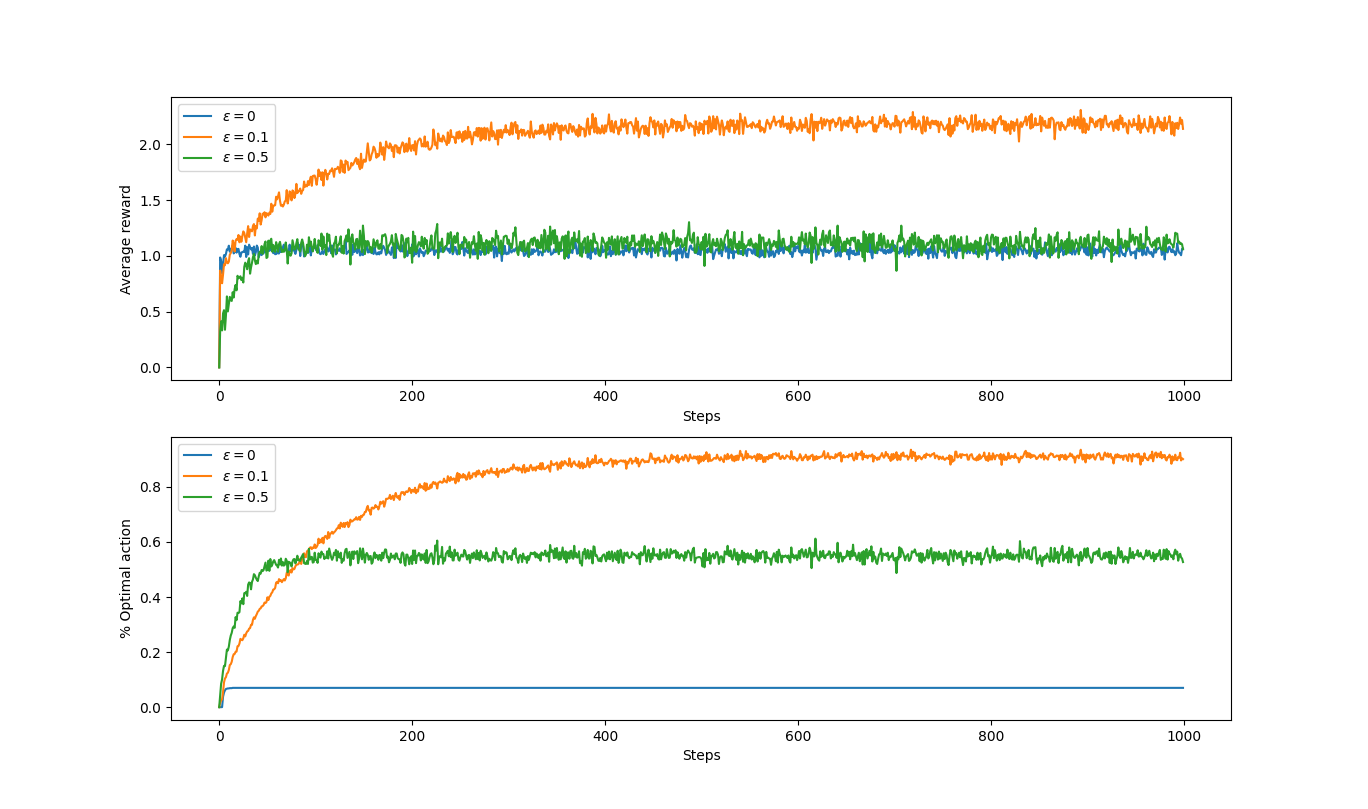
\includegraphics[width = 0.95 \textwidth]{1.4.1.png}
    \caption
    {
        Average performance of $\varepsilon$-greedy action-value methods on the $10$-armed testbed.
        These data are averages over $1000$ runs with different bandit problems.
        All methods used sample averages as their action-value estimates.
    }
    \label{fig:3}
\end{figure}

\end{solution}

% --------------------------------------------------------------------------------
